% Options for packages loaded elsewhere
\PassOptionsToPackage{unicode}{hyperref}
\PassOptionsToPackage{hyphens}{url}
%
\documentclass[
]{article}
\usepackage{lmodern}
\usepackage{amssymb,amsmath}
\usepackage{ifxetex,ifluatex}
\ifnum 0\ifxetex 1\fi\ifluatex 1\fi=0 % if pdftex
  \usepackage[T1]{fontenc}
  \usepackage[utf8]{inputenc}
  \usepackage{textcomp} % provide euro and other symbols
\else % if luatex or xetex
  \usepackage{unicode-math}
  \defaultfontfeatures{Scale=MatchLowercase}
  \defaultfontfeatures[\rmfamily]{Ligatures=TeX,Scale=1}
\fi
% Use upquote if available, for straight quotes in verbatim environments
\IfFileExists{upquote.sty}{\usepackage{upquote}}{}
\IfFileExists{microtype.sty}{% use microtype if available
  \usepackage[]{microtype}
  \UseMicrotypeSet[protrusion]{basicmath} % disable protrusion for tt fonts
}{}
\makeatletter
\@ifundefined{KOMAClassName}{% if non-KOMA class
  \IfFileExists{parskip.sty}{%
    \usepackage{parskip}
  }{% else
    \setlength{\parindent}{0pt}
    \setlength{\parskip}{6pt plus 2pt minus 1pt}}
}{% if KOMA class
  \KOMAoptions{parskip=half}}
\makeatother
\usepackage{xcolor}
\IfFileExists{xurl.sty}{\usepackage{xurl}}{} % add URL line breaks if available
\IfFileExists{bookmark.sty}{\usepackage{bookmark}}{\usepackage{hyperref}}
\hypersetup{
  pdftitle={CPI Analysis},
  pdfauthor={Zachary Palmore},
  hidelinks,
  pdfcreator={LaTeX via pandoc}}
\urlstyle{same} % disable monospaced font for URLs
\usepackage[margin=1in]{geometry}
\usepackage{color}
\usepackage{fancyvrb}
\newcommand{\VerbBar}{|}
\newcommand{\VERB}{\Verb[commandchars=\\\{\}]}
\DefineVerbatimEnvironment{Highlighting}{Verbatim}{commandchars=\\\{\}}
% Add ',fontsize=\small' for more characters per line
\usepackage{framed}
\definecolor{shadecolor}{RGB}{248,248,248}
\newenvironment{Shaded}{\begin{snugshade}}{\end{snugshade}}
\newcommand{\AlertTok}[1]{\textcolor[rgb]{0.94,0.16,0.16}{#1}}
\newcommand{\AnnotationTok}[1]{\textcolor[rgb]{0.56,0.35,0.01}{\textbf{\textit{#1}}}}
\newcommand{\AttributeTok}[1]{\textcolor[rgb]{0.77,0.63,0.00}{#1}}
\newcommand{\BaseNTok}[1]{\textcolor[rgb]{0.00,0.00,0.81}{#1}}
\newcommand{\BuiltInTok}[1]{#1}
\newcommand{\CharTok}[1]{\textcolor[rgb]{0.31,0.60,0.02}{#1}}
\newcommand{\CommentTok}[1]{\textcolor[rgb]{0.56,0.35,0.01}{\textit{#1}}}
\newcommand{\CommentVarTok}[1]{\textcolor[rgb]{0.56,0.35,0.01}{\textbf{\textit{#1}}}}
\newcommand{\ConstantTok}[1]{\textcolor[rgb]{0.00,0.00,0.00}{#1}}
\newcommand{\ControlFlowTok}[1]{\textcolor[rgb]{0.13,0.29,0.53}{\textbf{#1}}}
\newcommand{\DataTypeTok}[1]{\textcolor[rgb]{0.13,0.29,0.53}{#1}}
\newcommand{\DecValTok}[1]{\textcolor[rgb]{0.00,0.00,0.81}{#1}}
\newcommand{\DocumentationTok}[1]{\textcolor[rgb]{0.56,0.35,0.01}{\textbf{\textit{#1}}}}
\newcommand{\ErrorTok}[1]{\textcolor[rgb]{0.64,0.00,0.00}{\textbf{#1}}}
\newcommand{\ExtensionTok}[1]{#1}
\newcommand{\FloatTok}[1]{\textcolor[rgb]{0.00,0.00,0.81}{#1}}
\newcommand{\FunctionTok}[1]{\textcolor[rgb]{0.00,0.00,0.00}{#1}}
\newcommand{\ImportTok}[1]{#1}
\newcommand{\InformationTok}[1]{\textcolor[rgb]{0.56,0.35,0.01}{\textbf{\textit{#1}}}}
\newcommand{\KeywordTok}[1]{\textcolor[rgb]{0.13,0.29,0.53}{\textbf{#1}}}
\newcommand{\NormalTok}[1]{#1}
\newcommand{\OperatorTok}[1]{\textcolor[rgb]{0.81,0.36,0.00}{\textbf{#1}}}
\newcommand{\OtherTok}[1]{\textcolor[rgb]{0.56,0.35,0.01}{#1}}
\newcommand{\PreprocessorTok}[1]{\textcolor[rgb]{0.56,0.35,0.01}{\textit{#1}}}
\newcommand{\RegionMarkerTok}[1]{#1}
\newcommand{\SpecialCharTok}[1]{\textcolor[rgb]{0.00,0.00,0.00}{#1}}
\newcommand{\SpecialStringTok}[1]{\textcolor[rgb]{0.31,0.60,0.02}{#1}}
\newcommand{\StringTok}[1]{\textcolor[rgb]{0.31,0.60,0.02}{#1}}
\newcommand{\VariableTok}[1]{\textcolor[rgb]{0.00,0.00,0.00}{#1}}
\newcommand{\VerbatimStringTok}[1]{\textcolor[rgb]{0.31,0.60,0.02}{#1}}
\newcommand{\WarningTok}[1]{\textcolor[rgb]{0.56,0.35,0.01}{\textbf{\textit{#1}}}}
\usepackage{graphicx}
\makeatletter
\def\maxwidth{\ifdim\Gin@nat@width>\linewidth\linewidth\else\Gin@nat@width\fi}
\def\maxheight{\ifdim\Gin@nat@height>\textheight\textheight\else\Gin@nat@height\fi}
\makeatother
% Scale images if necessary, so that they will not overflow the page
% margins by default, and it is still possible to overwrite the defaults
% using explicit options in \includegraphics[width, height, ...]{}
\setkeys{Gin}{width=\maxwidth,height=\maxheight,keepaspectratio}
% Set default figure placement to htbp
\makeatletter
\def\fps@figure{htbp}
\makeatother
\setlength{\emergencystretch}{3em} % prevent overfull lines
\providecommand{\tightlist}{%
  \setlength{\itemsep}{0pt}\setlength{\parskip}{0pt}}
\setcounter{secnumdepth}{-\maxdimen} % remove section numbering
\usepackage{booktabs}
\usepackage{longtable}
\usepackage{array}
\usepackage{multirow}
\usepackage{wrapfig}
\usepackage{float}
\usepackage{colortbl}
\usepackage{pdflscape}
\usepackage{tabu}
\usepackage{threeparttable}
\usepackage{threeparttablex}
\usepackage[normalem]{ulem}
\usepackage{makecell}
\usepackage{xcolor}
\ifluatex
  \usepackage{selnolig}  % disable illegal ligatures
\fi

\title{CPI Analysis}
\author{Zachary Palmore}
\date{5/16/2021}

\begin{document}
\maketitle

\hypertarget{abstract}{%
\subsection{Abstract}\label{abstract}}

Businesses, governments, and consumers in the United States all rely on
some aspect of the consumer price index (CPI) when making financial
decisions. There is evidence to suggest that improperly measuring this
statistic by margins as small as 1.1\% could result in trillions of
dollars lost through government spending. This notion ties into the
economic behavior of businesses and consumers quite intuitively and yet,
we rely on models that predict using data on business and consumer
behavior that largely differs in our society today. Furthermore, recent
studies have identified a stabilization in the rate of inflation (which
is found through the CPI) since about 1980. This phenomenon has created
a dichotomy in the rate of change in prices of consumer goods and
services in which CPI estimates earlier than 1960 follow one pattern and
the estimates after 1980 follow another separate pattern. Through
univariate simple linear regression techniques we developed a
contemporary model that exploits the dichotomous nature of these
statistics and we attempt to prove that the holistic use of historical
data does not accurately capture the behavior of modern society nor does
it aid in its prediction.

\hypertarget{key-words}{%
\subsection{Key Words}\label{key-words}}

\hypertarget{introduction}{%
\subsection{Introduction}\label{introduction}}

There are a plethora of entities dedicated, at least in part, to
interpreting or predicting the Consumer Price Index (CPI) and rightfully
so. An accurate understanding of these statistics offers private and
public businesses and governing bodies alike the opportunity to make
better fiscal decisions such as when and how much to adjust interest
rates, allocate funds, control investments, and raise wages to name a
few. Inflation, another highly valued metric for all lending
institutions and consumers with credit investments, is found directly
from the change in CPI, further increasing its value. As stated in the
Journal of Economic Perspectives, ``Accurately measuring prices and
their rate of change, inflation, is central to almost every economic
issue.''

The Economic Research Service of the United States Department of
Agriculture and National Academy of Sciences has written since at least
2006 that reevaluating how the government measures poverty using a new
cost of living estimate that utilizes aspects of CPI would elucidate the
true nature of impoverished areas and would change who our algorithms
consider poor. This study highlights the necessity for new measures in
identifying groups of people who need the aid most which thereby reduces
currently undetected systemic injustices, reduces waste, and helps to
eliminate poverty. In short, use of the CPI in conjunction with other
metrics would make each dollar spent on programs like medicare,
medicaid, and other welfare assistance programs stretch farther. Due to
the Bureau of Labor Statistics' collection of consumer prices, officials
can accurately estimate the price of goods and in some regards, it may
also serve as a reasonable estimation of the cost of living for
individuals. Although, caution should be heeded for those who use the
CPI in this manner as its functionality plummets when applied broadly
and vastly as a discrete inflation measure. Of course, this is entirely
reliant on the validity of the CPI.

One study by an advisory committee established by the Senate Finance
Committee pursuant to a Senate Resolution and documented in the Journal
of Economic Perspectives found that ``Over a dozen years, the cumulative
additional national debt from overindexing the budget would amount to
more than \$1 trillion.'' In the same paper, they found the true CPI
value was only 1.1 percentage points over on average per year with a
range of 0.8 to 1.6 average percentage points per year. A minor
difference that in essence meant a CPI reported to be 3 percent, was
actually closer to 2 percent. However, this is not to say that the CPI
is any less valuable.

When measuring geographic variations in the cost of living to
cross-examine with the academic performance of children, the effects of
CPI when used as an indicator for the cost of living (COL) have
suggested higher costs were associated with lower achievement.
Simultaneously, investments in resources for those same children
resulted in better outcomes (often through academic scores) for children
in lower-income families. This relationship between the CPI and COL thus
has significant implications for assessing and improving the academic
performance of those in lower-income brackets, but the reasons to
understand and predict CPI do not stop there.

Regular updates of the CPI offer invaluable information that is central
to controlling for economic stability and enacting policies that benefit
society. Whether the entities are considering interest rates, monetary
accountability, or even education, the CPI has an integral role to play
and its accuracy is imperative to support wise decision making. For
these reasons, we attempt to build a model that captures the bulk of
information crucial in these efforts in today's economic environment
with a different approach during model development.

\hypertarget{literature-review}{%
\subsection{Literature Review}\label{literature-review}}

Previous research has shown that difficulties in modeling the CPI mostly
stem from the inherently unpredictable nature of inflation and consumer
prices. This phenomenon is also known as volatility. The agglomeration
of changes in prices of consumer goods and services across the US
contains an immense diversity of factors influencing those prices.
Consider, for example, the cost of water utilities between desert
climates such as in Arizona, New Mexico, and Nevada, with the relatively
water rich humid subtropical areas of Mississippi, Alabama, and
Louisiana. Holding relative demand constant, the cost in utilities to
collect or extract, maintain and deliver the supply of this resource
will vary considerably and thus, their prices fluctuate according to
largely separate variables. Keep in mind this is merely one fluctuating
consumer good in a basket of over 80,000 items.

According to the Bureau of Labor Statistics and several other
nongovernmental agencies, over the lifetime of the Federal Reserve
System (Fed) there has been a concerted effort to keep the inflation
rate low. Recall that this inflation rate is determined by finding the
change in CPI over time and recorded as an increase or decrease in each
calculation based only on the previous value. In this endeavor, the
system tends to focus on nonvolatile components which they call the core
inflation rate. Studies based on this core inflation rate (which
generally excludes food and energy utilities, though not exclusively)
have shown that modeling both goods and services ``have not fared well
in general.'' One justifiable reason that aggregation of this kind tends
to reflect poorly on model testing is that the core inflation measure
used by the Fed does not downselect the consumer goods or services well
enough to observe separate inflationary expectations. Doing so may also
result in another conundrum, that further reduction is necessary until
isolated groups all share distinctly similar volatility in their CPI.
Thus, an alternative modeling technique has been proposed.

As published in the Journal of Current Issues in Economics and Finance,
several researchers split the data into two groups, one that models the
CPI for goods, and one model for services with a critical success: more
accurate predictions. With this novel modeling process they captured
reality better than traditional core inflation models and were able to
discover the behavior of each group and its dependencies in more detail.
The observed CPI of goods depended on short-term expectations and import
prices, while services depended on long-term expectation and leeway of
the domestic labor market. Moreover, composite CPI models like this
improved the prediction without the use of additional external factors
when measured through inflationary reactions.

Today, the Phillips Inflation Curve Forecast remains the most useful
macroeconomic model when interpreting or predicting inflation with this
univariate model outperforming multivariate counterparts. However, their
performance is episodic, limiting their ability to perform well
continuously. Some also refer to these more novel models as New
Keynesian Phillips Curves (NKPC) models, and broadly speaking they
employ the use of an activity variable, which often simply means they
consider historical CPI values.

Evidence to characterize the backward-looking Phillips Inflation Curve
has shown that hawkish monetary policy approaches tend to `` trigger an
endogenous anchoring of agents' subjective inflation forecasts'' and
offer ``a coherent explanation for all of the observed changes in U.S.
inflation behavior.'' The literature also indicates that volatility in
CPI has decreased since the 1980's along with the persistence of US
inflation to increase. Those familiar with the relation of inflation
rates with the output gap have noted that stability in the Philips
Inflation Curve Forecasts has resurfaced from U.S. data since 1980.
Additionally, studies done with this backward-looking Phillips model
that improve their choice of anchoring (or benchmark) years have been
shown to produce statistically significant ``estimated structural slope
parameter in the NKPC'' for the range of years 1960-2019.

\hypertarget{methodology}{%
\subsection{Methodology}\label{methodology}}

In accordance with studies based on NKPC models, we intend to develop a
univariate simple linear regression model for the CPI. This model will
differ from others in its segmentation. As previously stated, two
stabilized periods of years seem to extend from about 1913 to 1960, and
1980 onwards. We intend to divulge the relationship of these two
segmented periods as their own separate models.

Data is sourced from the BLS and contains monthly CPI estimates for each
year over the range 1913-2014. The benchmark for which the entire data
set is evaluated is the arithmetic mean of the annual CPI for the
1982-1984. Data collection did not begin until 1913 via authorization
from Congress. Monthly estimates are given on the first of each month
and start with January 1, 1913. The final monthly estimate ends on
January 1, 2014. Inflation is calculated alongside CPI as a new variable
but remember, this is only a representative estimate of the change in
CPI values from one month to the next. Inflation calculations did not
begin until May 1, 2014.

\hypertarget{experimentation-and-results}{%
\subsection{Experimentation and
Results}\label{experimentation-and-results}}

Newer portions of the data were stored in reports released by the BLS
corresponding to the timespan between the first of May in 2014 to the
first of March in 2021. This data would only be used in evaluation of
the model performance statistics. All preceding data from the first of
May in 2014 backwards, was made available in a comma delimited format
and was extracted from the open source API by data.io for hosting
purposes and reproducibility. See the appendix for further descriptions
of exactly how this data was extracted. The first few observations are
shown.

\begin{table}[!h]

\caption{\label{tab:unnamed-chunk-3}CPI Raw Data Initial Observations}
\centering
\begin{tabular}[t]{lrr}
\toprule
Date & Index & Inflation\\
\midrule
\cellcolor{gray!6}{1913-01-01} & \cellcolor{gray!6}{9.8} & \cellcolor{gray!6}{NA}\\
1913-02-01 & 9.8 & 0.00\\
\cellcolor{gray!6}{1913-03-01} & \cellcolor{gray!6}{9.8} & \cellcolor{gray!6}{0.00}\\
1913-04-01 & 9.8 & 0.00\\
\cellcolor{gray!6}{1913-05-01} & \cellcolor{gray!6}{9.7} & \cellcolor{gray!6}{-1.02}\\
\addlinespace
1913-06-01 & 9.8 & 1.03\\
\bottomrule
\end{tabular}
\end{table}

Our first step in this experiment is the separation of the data into two
distinct segments, and to do so we first justify the need and
approximate the periods with which to draw from. This is merely a check
on the literature but we can see the results as a scatterplot. To assist
in the attempted segmentation based on mathematical behavior, we do not
add a trend to the plot at this time. Inflation is highlighted on a
continuous scale for each month within the range.

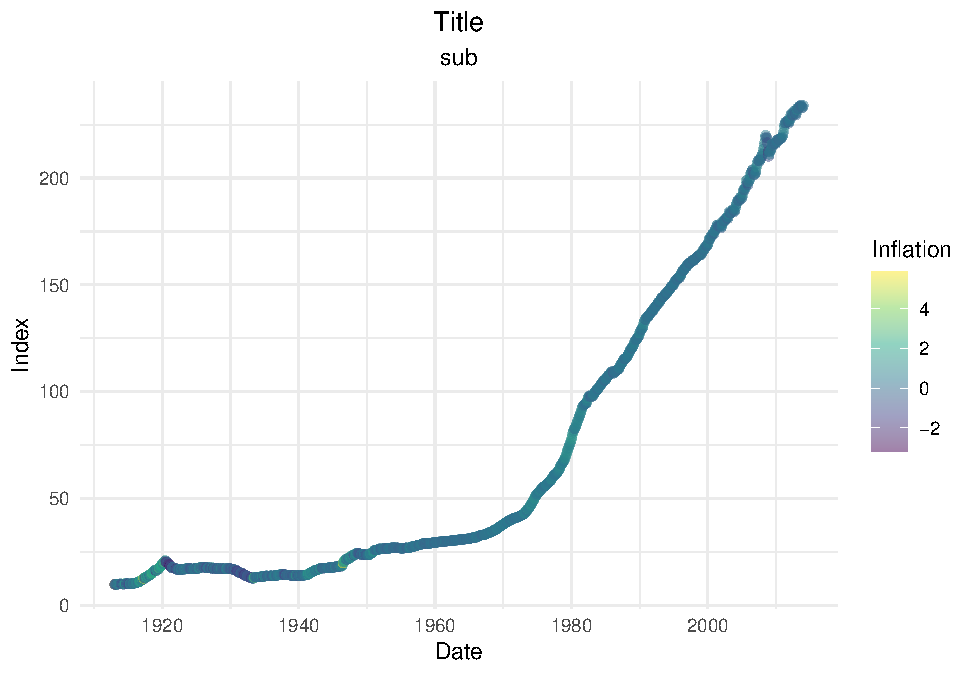
\includegraphics{CPIAnalysis_files/figure-latex/unnamed-chunk-4-1.pdf}

Showing the distribution of CPI from 1913 to 2014 gives us insight into
the two groups, because prior to the late 1960's the data appear to fall
in line with steady slope of some caliber while the data after the late
1970's follows a much steeper incline. This is our basis for
segmentation. Meanwhile, the inflation colored at this scale is
practically constant except for a jump in the 1920's and a rapid
exponentiation of inflation for the late 1960's to the early 1980's. We
examine this further at two closer scales.

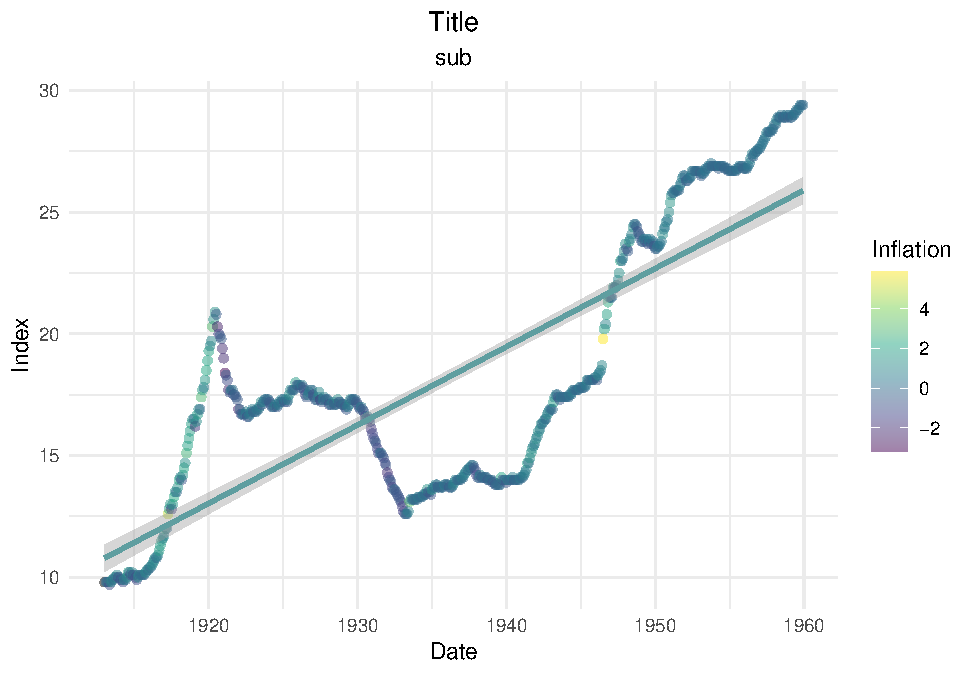
\includegraphics{CPIAnalysis_files/figure-latex/unnamed-chunk-5-1.pdf}

By filtering the data to include only those CPI values that were less
than the first of January in 1960, a new story emerges. It is clear that
the slope is not constant. There is a substantial amount of variation in
the CPI and inflation throughout the 1913 - 1960 range. Presumably, this
is due to differences in fiscal policy that occurred before 1920 and
thereafter when the Great Depression hit the United States. Needless to
say, prediction based on a model of this data would result in less than
ideal conditions for understanding future CPI and inflation rates.

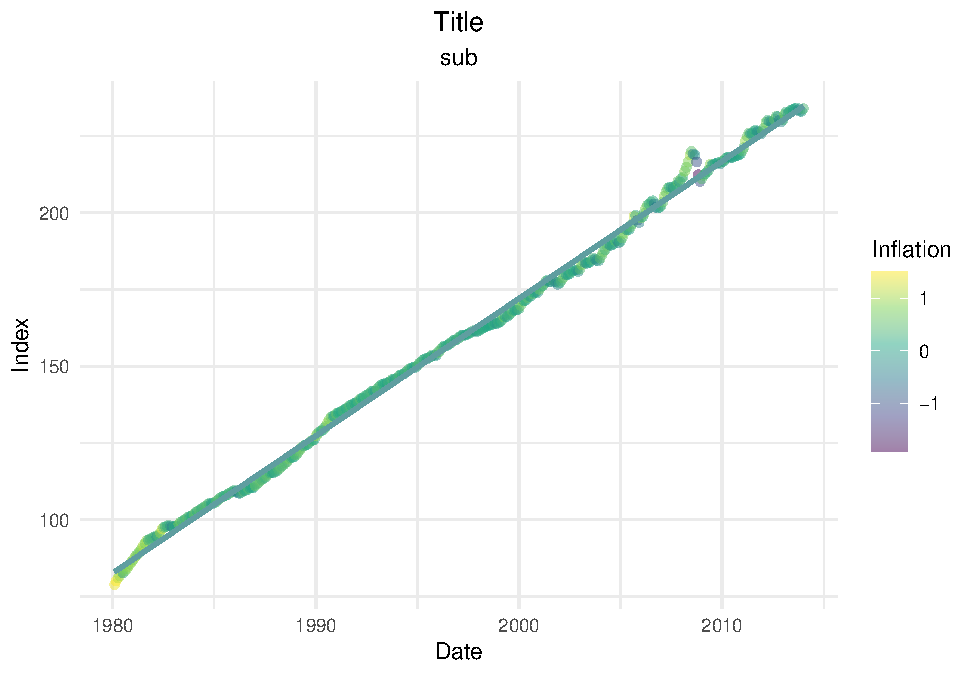
\includegraphics{CPIAnalysis_files/figure-latex/unnamed-chunk-6-1.pdf}

Filtering from the first of January in 1980 until the upper limit of our
data range on the first of January in 2014, we get a near constant
slope. There is only one minor `blip' or divergence from this expected
trend around 2008. Arguably, this is a better segment to make
predictions and draw recent conclusions from. A major cause of the
resultant blip is likely the Great Recession which certainly resulted in
an intense fluctuation of many consumer goods.

Model development is straightforward using the segmentation date ranges
as selection, or specifically filtering criteria for our first
pre-seventies date range to run through our simple linear regression. We
then run diagnostic plots to evaluate our assumptions. Given the
somewhat poor linearity we should expect a poorly fitted residual vs
fitted plot, if there is a well enough presence at all. Judging from the
previous scatterplot and linear regression overlay, we know very few CPI
values were solid hits on the trend. A valid normality may also be a
concern.

\begin{verbatim}
## 
## Call:
## lm(formula = Index ~ Date, data = g1)
## 
## Residuals:
##    Min     1Q Median     3Q    Max 
## -5.739 -3.305  1.050  2.773  7.729 
## 
## Coefficients:
##              Estimate Std. Error t value Pr(>|t|)    
## (Intercept) 2.912e+01  3.687e-01   78.98   <2e-16 ***
## Date        8.808e-04  2.790e-05   31.57   <2e-16 ***
## ---
## Signif. codes:  0 '***' 0.001 '**' 0.01 '*' 0.05 '.' 0.1 ' ' 1
## 
## Residual standard error: 3.284 on 562 degrees of freedom
## Multiple R-squared:  0.6394, Adjusted R-squared:  0.6388 
## F-statistic: 996.6 on 1 and 562 DF,  p-value: < 2.2e-16
\end{verbatim}

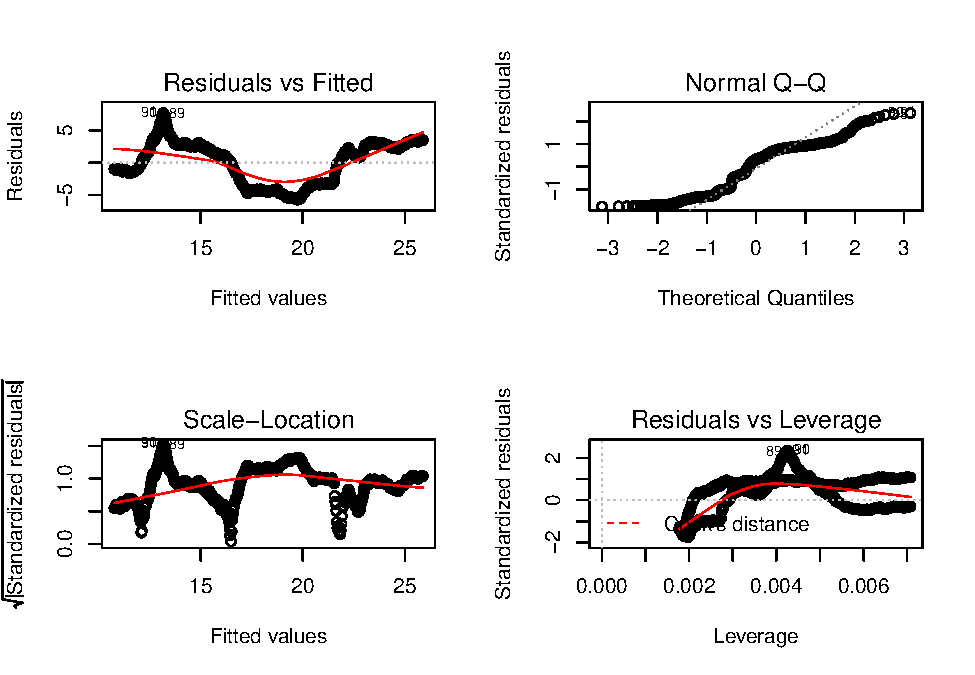
\includegraphics{CPIAnalysis_files/figure-latex/unnamed-chunk-7-1.pdf}

As expected, linearity is poor and normality is not present. While we
could attempt to overlook the normality of the plot through various
transformations, such efforts would be wasted as there is likely no
reasonable transformation that would not completely change the meaning
of the data. When even the Scale-Location and Residual vs Leverage plot
indicates the presence of highly influential values, there is little
hope to piecemeal the variations from this range into something
practical. Instead, we should make note of this pattern as it confirms
our thoughts that data prior to the first of January in 1960 does indeed
behave differently than any expectations of linearity. We repeat this
preliminary modeling process on the data from 1980 onward.

\begin{verbatim}
## 
## Call:
## lm(formula = Index ~ Date, data = g2)
## 
## Residuals:
##     Min      1Q  Median      3Q     Max 
## -5.2504 -1.8410  0.2805  1.5275  9.9303 
## 
## Coefficients:
##              Estimate Std. Error t value Pr(>|t|)    
## (Intercept) 3.798e+01  3.293e-01   115.3   <2e-16 ***
## Date        1.224e-02  3.134e-05   390.4   <2e-16 ***
## ---
## Signif. codes:  0 '***' 0.001 '**' 0.01 '*' 0.05 '.' 0.1 ' ' 1
## 
## Residual standard error: 2.269 on 406 degrees of freedom
## Multiple R-squared:  0.9973, Adjusted R-squared:  0.9973 
## F-statistic: 1.524e+05 on 1 and 406 DF,  p-value: < 2.2e-16
\end{verbatim}

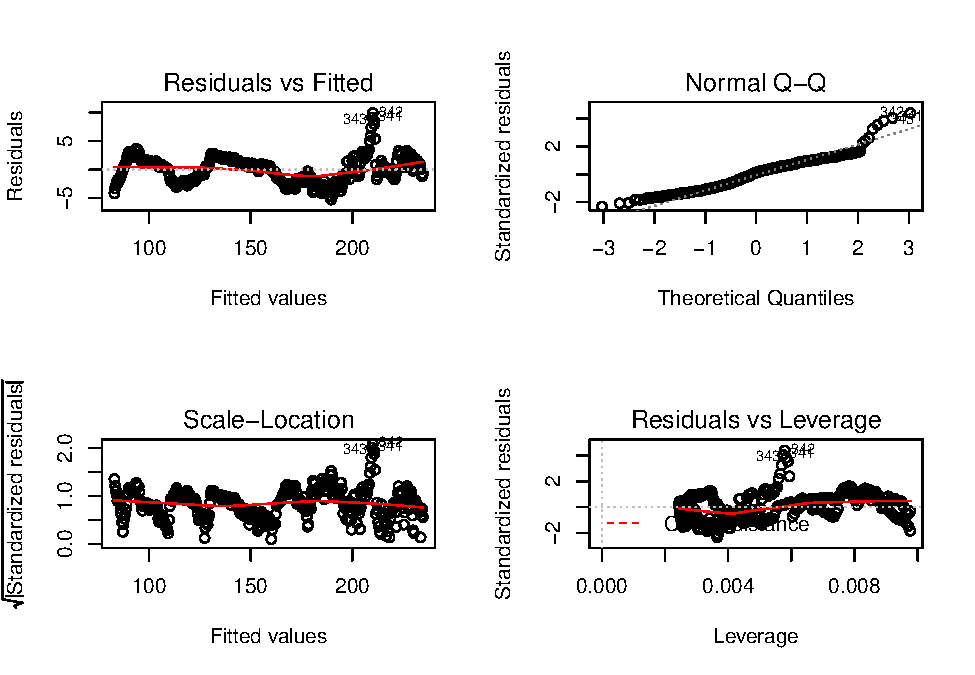
\includegraphics{CPIAnalysis_files/figure-latex/unnamed-chunk-8-1.pdf}

While the normality of the distribution is still questionable and there
are a few CPI values that diverge from expectations in our Residuals vs
Leverage plot, this data set gives us something we can work with. We
recognize that this data is inherently variable and as such may never be
truly Bayesian in its distribution. Transformations may be beneficial,
in this case, when trying to explain the relationship of CPI over time.
To better assess this relationship in an attempt to predict its behavior
more accurately, we should split this data into training and testing
data sets for model development. We also use a Bayesian classifier to
determine the most appropriate transformation on this training data.

\begin{verbatim}
## Best Normalizing transformation with 288 Observations
##  Estimated Normality Statistics (Pearson P / df, lower => more normal):
##  - arcsinh(x): 1.3294
##  - Box-Cox: 1.2658
##  - Center+scale: 1.1924
##  - Exp(x): 34.7778
##  - Log_b(x+a): 1.3294
##  - orderNorm (ORQ): 1.2422
##  - sqrt(x + a): 1.2394
##  - Yeo-Johnson: 1.268
## Estimation method: Out-of-sample via CV with 10 folds and 5 repeats
##  
## Based off these, bestNormalize chose:
## center_scale(x) Transformation with 288 nonmissing obs.
##  Estimated statistics:
##  - mean (before standardization) = 158.5135 
##  - sd (before standardization) = 43.79097
\end{verbatim}

Perhaps ironically based on this classifier, centering and scaling the
data is our best option from a host of statistical operations even
though it will not adjust normality of residuals. These operations
include but are not limited to Box-Cox, Yeo-Johnson, orderNorm, and sqrt
which were each close runner-up transformations. We perform these on our
newest training data with 70\% of the original CPI dates and values. The
results are shown:

\begin{verbatim}
## 
## Call:
## lm(formula = Index ~ Date, data = train)
## 
## Residuals:
##       Min        1Q    Median        3Q       Max 
## -0.118151 -0.043081  0.005851  0.036281  0.229216 
## 
## Coefficients:
##               Estimate Std. Error t value Pr(>|t|)    
## (Intercept) -2.749e+00  9.113e-03  -301.7   <2e-16 ***
## Date         2.790e-04  8.695e-07   320.9   <2e-16 ***
## ---
## Signif. codes:  0 '***' 0.001 '**' 0.01 '*' 0.05 '.' 0.1 ' ' 1
## 
## Residual standard error: 0.05272 on 286 degrees of freedom
## Multiple R-squared:  0.9972, Adjusted R-squared:  0.9972 
## F-statistic: 1.03e+05 on 1 and 286 DF,  p-value: < 2.2e-16
\end{verbatim}

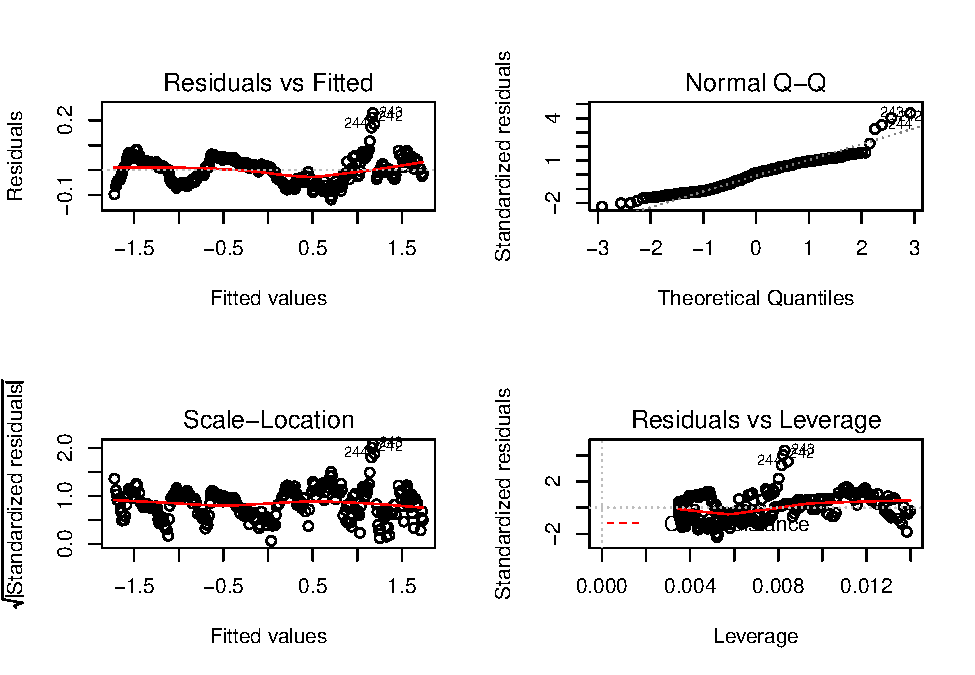
\includegraphics{CPIAnalysis_files/figure-latex/unnamed-chunk-10-1.pdf}

Normality does not change, but the distance of our red trendlines and
axis values appear to have shrunk in size, which we suspect benefits the
linearity of Residuals vs Fitted as well as our Scale-Location and
Residuals vs Leverage plots. At the expense of .1\% of our \(R^2\)
value, we have successfully reduced the standard error in this model to
near 0.05 down from 2.7. We add these statistics to our table and
calculate the errors in every prediction, its magnitude, the average
error of every prediction, and compute the root mean squared error in
subsequent steps.

\begin{table}[!h]

\caption{\label{tab:unnamed-chunk-11}Scaled Contemporary Model Test Statistics}
\centering
\begin{tabular}[t]{lllllll}
\toprule
\cellcolor{gray!6}{Date} & \cellcolor{gray!6}{1980-02-01} & \cellcolor{gray!6}{1980-04-01} & \cellcolor{gray!6}{1980-05-01} & \cellcolor{gray!6}{1980-06-01} & \cellcolor{gray!6}{1980-09-01} & \cellcolor{gray!6}{1980-10-01}\\
Index & -1.818035 & -1.770080 & -1.751811 & -1.731259 & -1.701573 & -1.683304\\
\cellcolor{gray!6}{Inflation} & \cellcolor{gray!6}{1.41} & \cellcolor{gray!6}{1.12} & \cellcolor{gray!6}{0.99} & \cellcolor{gray!6}{1.10} & \cellcolor{gray!6}{0.84} & \cellcolor{gray!6}{0.95}\\
scaled.predicted & -1.721413 & -1.704673 & -1.696303 & -1.687654 & -1.661986 & -1.653616\\
\cellcolor{gray!6}{scaled.error} & \cellcolor{gray!6}{-0.09662188} & \cellcolor{gray!6}{-0.06540681} & \cellcolor{gray!6}{-0.05550821} & \cellcolor{gray!6}{-0.04360504} & \cellcolor{gray!6}{-0.03958658} & \cellcolor{gray!6}{-0.02968798}\\
\addlinespace
scaled.mag & 0.0093357882 & 0.0042780508 & 0.0030811617 & 0.0019013995 & 0.0015670974 & 0.0008813764\\
\cellcolor{gray!6}{scaled.eravg} & \cellcolor{gray!6}{0.002760148} & \cellcolor{gray!6}{0.002760148} & \cellcolor{gray!6}{0.002760148} & \cellcolor{gray!6}{0.002760148} & \cellcolor{gray!6}{0.002760148} & \cellcolor{gray!6}{0.002760148}\\
scaled.rmse & 0.05253711 & 0.05253711 & 0.05253711 & 0.05253711 & 0.05253711 & 0.05253711\\
\bottomrule
\end{tabular}
\end{table}

Our resultant model produces values that fall almost exactly on the
regression line, indicating a near perfect fit for an imperfect data
set. Inflation values are again highlighted for reference on a
continuous scale. Notice how the points of change in inflation did not
change, only the location of points on the plot and the scale of the
axes. Over the same time frame, our scaled prediction values perform
marginally better than the original contemporary model.

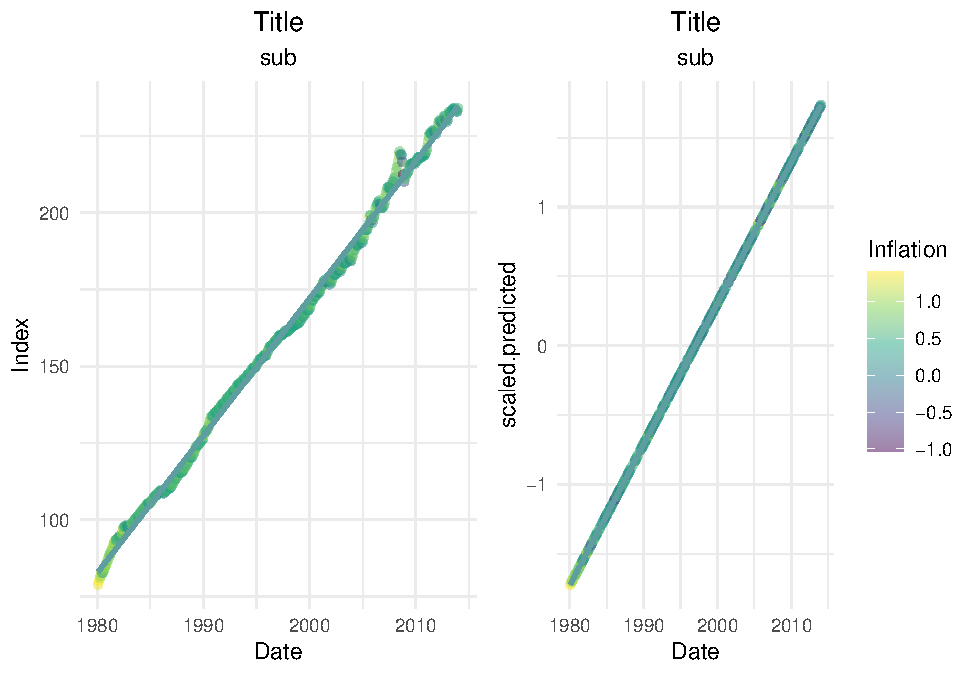
\includegraphics{CPIAnalysis_files/figure-latex/unnamed-chunk-12-1.pdf}

As a final check, we review the standard errors of each prediction and
its magnitude as both density plots and histograms. At this scale,
nearly all errors occur between -0.1 and 0.1 with the magnitude of those
errors rarely ever having an occurrence greater than .01. This is good
news for the contemporary model hypothesis.

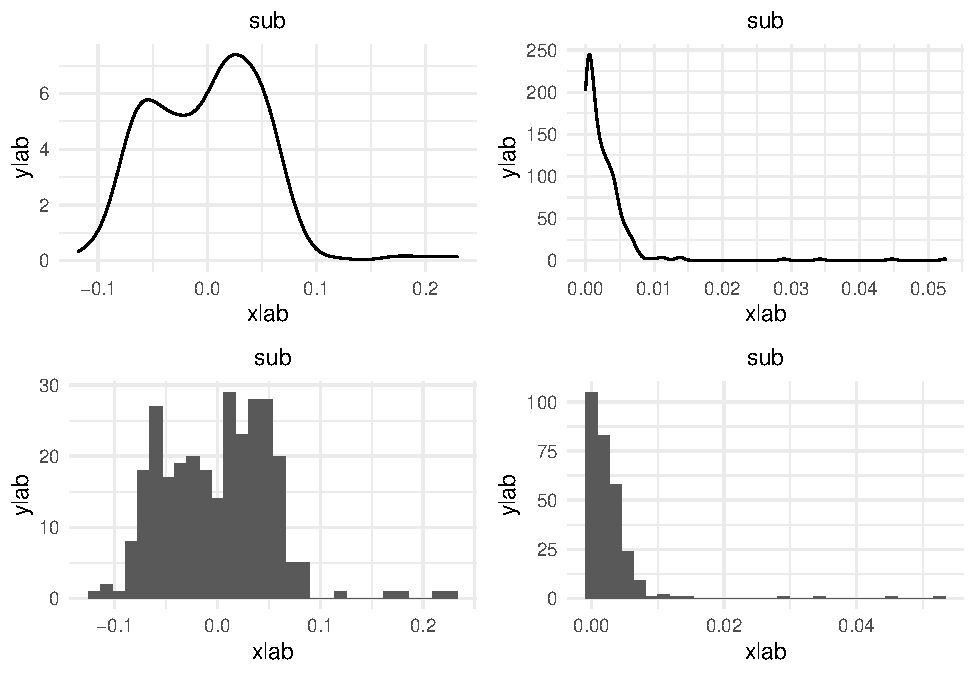
\includegraphics{CPIAnalysis_files/figure-latex/unnamed-chunk-13-1.pdf}

\hypertarget{discussion-and-conclusion}{%
\subsection{Discussion and Conclusion}\label{discussion-and-conclusion}}

Given recent citations in literature about the significant level of new
stability in inflation measures we hypothesized that CPI data from the
first of January in 1980 through the latest adjusted points we could
find in 2014 would show that a contemporary model is justified for
predicting CPI and its related affiliate statistics. In our experiment
the old-fashioned model failed all but one of the assumptions of linear
regression (leverage remained) and was only able to explain about 63.8\%
of the data with a t-statistic of 79.69 on 563 degrees of freedom (DF)
and was statistically significant beyond an alpha level of 0.001.
Meanwhile, our contemporary model explained 99.7\% of the data, with a
p-value less than 0.001 and a t-statistic of 72.95 with 407 DF. Lastly,
after the data underwent a 70-30 split with a center-scale
transformation, our scaled contemporary model improved upon these scores
by reducing the standard error of the contemporary model to 0.053 on 286
degrees of freedom while all other test statistics remained nearly
unchanged. Our final root mean squared error for this scaled
contemporary model was 0.0525, with an mean error of 0.0028, and no
error larger than 0.229. Based on this experiment modeling the segmented
time periods, there is evidence to support making predictions on the
basis that data prior to 1980 is impractical for prediction in modern
times.

\hypertarget{references}{%
\subsection{References}\label{references}}

\(^{1}\)Baker, E. S. (2014, May). Modeling core inflation: Considering
goods and services separately. Retrieved from
\url{https://www.bls.gov/opub/mlr/2014/beyond-bls/pdf/modeling-core-inflation-considering-goods-and-services-separately.pdf}

\(^{2}\)Board of Governors, F. (2021, May 03). Effective federal funds
rate. Retrieved from \url{https://fred.stlouisfed.org/series/FEDFUNDS}

\(^{3}\)Brissimis, S. N., Economic Research Department, Bank of Greece,
\& Magginas, N. S., Department of Economics, University of Piraeus.
(2008). Inflation Forecasts and the New Keynesian Phillips Curve.
International Journal of Central Banking, (13).
\url{doi:https://www.ijcb.org/journal/ijcb08q2a1.pdf}

\(^{4}\)Bureau of Labor Statistics. (2021, May 12). Archived consumer
price index supplemental files. Retrieved from
\url{https://www.bls.gov/cpi/tables/supplemental-files/home.htm}

\(^{5}\)Chao, E. L., U.S. Department of Labor, \& Utgoff, K. P., U.S.
Bureau of Labor Statistics. (2006, May). 100 Years of U.S. Consumer
Spending: Data for the Nation, New York City, and Boston. Retrieved from
\url{https://www.bls.gov/opub/100-years-of-u-s-consumer-spending.pdf}

\(^{6}\)Chien, N., \& Mistry, R. (2013). Geographic variations in cost
of living: Associations with family and child well-being. Retrieved May
22, 2021, from
\url{https://www.ncbi.nlm.nih.gov/pmc/articles/PMC3509251/}

\(^{7}\)Consumer price index frequently asked questions. (2021).
Retrieved from \url{https://www.bls.gov/cpi/questions-and-answers.htm}

\(^{8}\)Data source from data.io: Consumer Price Index for All Urban
Consumers (CPI-U) from U.S. Department Of Labor Bureau of Labor
Statistics. Retrieved from using online link:
\url{https://pkgstore.datahub.io/core/cpi-us/8/datapackage.json}

\(^{9}\)DeSilver, D. (2020, May 30). How America's diet has changed over
time. Retrieved from
\url{https://www.pewresearch.org/fact-tank/2016/12/13/whats-on-your-table-how-americas-diet-has-changed-over-the-decades/}

\(^{10}\)Fernando, J. (2021, May 20). Consumer price index (cpi)
definition. Retrieved from
\url{https://www.investopedia.com/terms/c/consumerpriceindex.asp\#}:\textasciitilde:text=The\%20CPI\%20measures\%20the\%20average,services\%2C\%20commonly\%20known\%20as\%20inflation.\&text=The\%20quoted\%20inflation\%20rate\%20is,is\%20monthly\%2C\%20quarterly\%20or\%20yearly.

\(^{11}\)James H. Stock \& Mark W. Watson, 2008. ``Phillips curve
inflation forecasts,'' Conference Series ; {[}Proceedings{]}, Federal
Reserve Bank of Boston, vol.~53.

\(^{12}\)Jolliffe, D. (2006, November 01). Adjusting for living costs
can change who is considered poor. Retrieved from
\url{https://www.ers.usda.gov/amber-waves/2006/november/adjusting-for-living-costs-can-change-who-is-considered-poor/}

\(^{13}\)Jolliffe, D. (2006, November 01). Adjusting for Living Costs
Can Change Who Is Considered Poor. Retrieved May 21, 2021, from
\url{https://www.ers.usda.gov/amber-waves/2006/november/adjusting-for-living-costs-can-change-who-is-considered-poor/}

\(^{14}\)Jørgensen, Peter Lihn, Kevin J. Lansing. 2021. ``Anchored
Inflation Expectations and the Flatter Phillips Curve,'' Federal Reserve
Bank of San Francisco Working Paper 2019-27.
\url{https://doi.org/10.24148/wp2019-27}

\(^{15}\)Koba, M. (2013, May 01). Consumer price Index: CNBC Explains.
Retrieved from \url{https://www.cnbc.com/id/43769766}

\(^{16}\)Peach, R., Rich, R., \& Linder, M. H. (2013). The Parts Are
More Than the Whole: Separating Goods and Services to Predict Core
Inflation. Current Issues in Economics and Finance, 19(7).
\url{doi:https://www.newyorkfed.org/medialibrary/media/research/current_issues/ci19-7.pdf}

\(^{17}\)Staff. Bureau of Labor Statistics. (2021, May 19). Consumer
price index up 4.2 percent from April 2020 to April 2021. Retrieved from
\url{https://www.bls.gov/opub/ted/2021/consumer-price-index-up-4-2-percent-from-april-2020-to-april-2021.htm}

\(^{18}\)Stock, J. H., \& Watson, M. W. (2008). Phillips curve inflation
forecasts. National Bureau of Economic Research, 53, 14322nd ser.
\url{doi:10.3386/w14322}

\(^{19}\)Stock, J. H., \& Watson, M. W. (2019). Forecasting Inflation.
Retrieved from
\url{https://scholar.harvard.edu/files/stock/files/forecastinginflation.pdf}

\hypertarget{appendecies}{%
\subsection{Appendecies}\label{appendecies}}

\begin{Shaded}
\begin{Highlighting}[]
\FunctionTok{library}\NormalTok{(tesseract)}
\FunctionTok{library}\NormalTok{(magick)}
\FunctionTok{library}\NormalTok{(tidyverse)}
\FunctionTok{library}\NormalTok{(viridis)}
\FunctionTok{library}\NormalTok{(caret)}
\FunctionTok{library}\NormalTok{(pROC)}
\FunctionTok{library}\NormalTok{(bestNormalize)}
\FunctionTok{library}\NormalTok{(ggpubr)}
\FunctionTok{theme\_set}\NormalTok{(}\FunctionTok{theme\_minimal}\NormalTok{())}
\end{Highlighting}
\end{Shaded}

\begin{Shaded}
\begin{Highlighting}[]
\CommentTok{\# remove notes to download files individually from Git}
\CommentTok{\# specify correct file path otherwise it will not function properly }
\CommentTok{\# cpi1 \textless{}{-} tesseract\_download("https://raw.githubusercontent.com/palmorezm/msds/main/621/Final/cpi\_1913to1970.JPG", "C:/Users/Owner/Documents/Data/cpi1.jpg")}
\CommentTok{\# cpi2 \textless{}{-} tesseract\_download("https://raw.githubusercontent.com/palmorezm/msds/main/621/Final/cpi\_1971to2021.JPG", "C:/Users/Owner/Documents/Data/cpi1.jpg")}
\CommentTok{\# Image recognition}
\NormalTok{cpi1 }\OtherTok{\textless{}{-}} \FunctionTok{image\_read}\NormalTok{(}\StringTok{"C:/General/cpi1.jpg"}\NormalTok{)}
\NormalTok{cpi2 }\OtherTok{\textless{}{-}} \FunctionTok{image\_read}\NormalTok{(}\StringTok{"C:/General/cpi2.jpg"}\NormalTok{)}
\CommentTok{\# Cleanup and combine}
\NormalTok{ocr1 }\OtherTok{\textless{}{-}}\NormalTok{ cpi1 }\SpecialCharTok{\%\textgreater{}\%} 
  \FunctionTok{image\_resize}\NormalTok{(}\StringTok{"1200"}\NormalTok{) }\SpecialCharTok{\%\textgreater{}\%} 
  \FunctionTok{image\_trim}\NormalTok{() }\SpecialCharTok{\%\textgreater{}\%} 
  \FunctionTok{ocr}\NormalTok{()}
\NormalTok{ocr2 }\OtherTok{\textless{}{-}}\NormalTok{ cpi2 }\SpecialCharTok{\%\textgreater{}\%} 
  \FunctionTok{image\_resize}\NormalTok{(}\StringTok{"1200"}\NormalTok{) }\SpecialCharTok{\%\textgreater{}\%} 
  \FunctionTok{image\_trim}\NormalTok{() }\SpecialCharTok{\%\textgreater{}\%} 
  \FunctionTok{ocr}\NormalTok{()}
\FunctionTok{str\_extract}\NormalTok{(ocr1, }\StringTok{""}\NormalTok{)}
\CommentTok{\# remove notes to export}
\CommentTok{\# export as txt delimited by comma for ease of access}
\CommentTok{\# write.lines(ocr\_export, "C:/insert/file/path/here/for/local/machine)}
\end{Highlighting}
\end{Shaded}

\begin{Shaded}
\begin{Highlighting}[]
\NormalTok{cpi }\OtherTok{\textless{}{-}} \FunctionTok{read\_delim}\NormalTok{(}
  \StringTok{"https://raw.githubusercontent.com/palmorezm/msds/main/621/Final/cpi1\_1913\_present.txt"}\NormalTok{, }\StringTok{","}\NormalTok{)}
\FunctionTok{head}\NormalTok{(cpi)}
\end{Highlighting}
\end{Shaded}

\begin{Shaded}
\begin{Highlighting}[]
\NormalTok{cpi }\SpecialCharTok{\%\textgreater{}\%} 
  \FunctionTok{ggplot}\NormalTok{(}\FunctionTok{aes}\NormalTok{(Date, Index)) }\SpecialCharTok{+} \FunctionTok{geom\_point}\NormalTok{(}\FunctionTok{aes}\NormalTok{(}\AttributeTok{color=}\NormalTok{Inflation)) }\SpecialCharTok{+} 
  \FunctionTok{scale\_color\_viridis\_c}\NormalTok{(}\AttributeTok{aesthetics =} \FunctionTok{c}\NormalTok{(}\StringTok{"colour"}\NormalTok{, }\StringTok{"fill"}\NormalTok{), }\AttributeTok{option =} \StringTok{"D"}\NormalTok{, }\AttributeTok{alpha =}\NormalTok{ .}\DecValTok{5}\NormalTok{) }\SpecialCharTok{+} 
  \FunctionTok{labs}\NormalTok{(}\AttributeTok{title =} \StringTok{"Title"}\NormalTok{, }\AttributeTok{subtitle =} \StringTok{"sub"}\NormalTok{, }\AttributeTok{xlab=}\StringTok{"xlab"}\NormalTok{, }\AttributeTok{ylab=}\StringTok{"ylab"}\NormalTok{) }\SpecialCharTok{+} 
  \FunctionTok{theme}\NormalTok{(}\AttributeTok{plot.title =} \FunctionTok{element\_text}\NormalTok{(}\AttributeTok{hjust =}\NormalTok{ .}\DecValTok{5}\NormalTok{), }\AttributeTok{plot.subtitle =} \FunctionTok{element\_text}\NormalTok{(}\AttributeTok{hjust =}\NormalTok{ .}\DecValTok{5}\NormalTok{))}
\end{Highlighting}
\end{Shaded}

\begin{Shaded}
\begin{Highlighting}[]
\NormalTok{cpi }\SpecialCharTok{\%\textgreater{}\%} 
  \FunctionTok{filter}\NormalTok{(Date }\SpecialCharTok{\textless{}} \StringTok{"1960{-}01{-}01"}\NormalTok{) }\SpecialCharTok{\%\textgreater{}\%} 
  \FunctionTok{ggplot}\NormalTok{(}\FunctionTok{aes}\NormalTok{(Date, Index)) }\SpecialCharTok{+} \FunctionTok{geom\_point}\NormalTok{(}\FunctionTok{aes}\NormalTok{(}\AttributeTok{color=}\NormalTok{Inflation)) }\SpecialCharTok{+} 
  \FunctionTok{geom\_smooth}\NormalTok{(}\AttributeTok{method =} \StringTok{"lm"}\NormalTok{, }\AttributeTok{color=}\StringTok{"cadetblue"}\NormalTok{, }\AttributeTok{stat =} \StringTok{"smooth"}\NormalTok{, }\AttributeTok{se=}\ConstantTok{TRUE}\NormalTok{) }\SpecialCharTok{+}
  \FunctionTok{scale\_color\_viridis\_c}\NormalTok{(}\AttributeTok{aesthetics =} \FunctionTok{c}\NormalTok{(}\StringTok{"colour"}\NormalTok{, }\StringTok{"fill"}\NormalTok{), }\AttributeTok{option =} \StringTok{"D"}\NormalTok{, }\AttributeTok{alpha =}\NormalTok{ .}\DecValTok{5}\NormalTok{) }\SpecialCharTok{+} 
  \FunctionTok{labs}\NormalTok{(}\AttributeTok{title =} \StringTok{"Title"}\NormalTok{, }\AttributeTok{subtitle =} \StringTok{"sub"}\NormalTok{, }\AttributeTok{xlab=}\StringTok{"xlab"}\NormalTok{, }\AttributeTok{ylab=}\StringTok{"ylab"}\NormalTok{) }\SpecialCharTok{+} 
  \FunctionTok{theme}\NormalTok{(}\AttributeTok{plot.title =} \FunctionTok{element\_text}\NormalTok{(}\AttributeTok{hjust =}\NormalTok{ .}\DecValTok{5}\NormalTok{), }\AttributeTok{plot.subtitle =} \FunctionTok{element\_text}\NormalTok{(}\AttributeTok{hjust =}\NormalTok{ .}\DecValTok{5}\NormalTok{))}
\end{Highlighting}
\end{Shaded}

\begin{Shaded}
\begin{Highlighting}[]
\NormalTok{cpi }\SpecialCharTok{\%\textgreater{}\%} 
  \FunctionTok{filter}\NormalTok{(Date }\SpecialCharTok{\textgreater{}} \StringTok{"1980{-}01{-}01"}\NormalTok{) }\SpecialCharTok{\%\textgreater{}\%} 
  \FunctionTok{ggplot}\NormalTok{(}\FunctionTok{aes}\NormalTok{(Date, Index)) }\SpecialCharTok{+} \FunctionTok{geom\_point}\NormalTok{(}\FunctionTok{aes}\NormalTok{(}\AttributeTok{color=}\NormalTok{Inflation)) }\SpecialCharTok{+} 
  \FunctionTok{geom\_smooth}\NormalTok{(}\AttributeTok{method =} \StringTok{"lm"}\NormalTok{, }\AttributeTok{color=}\StringTok{"cadetblue"}\NormalTok{, }\AttributeTok{stat =} \StringTok{"smooth"}\NormalTok{, }\AttributeTok{se=}\ConstantTok{TRUE}\NormalTok{) }\SpecialCharTok{+}
  \FunctionTok{scale\_color\_viridis\_c}\NormalTok{(}\AttributeTok{aesthetics =} \FunctionTok{c}\NormalTok{(}\StringTok{"colour"}\NormalTok{, }\StringTok{"fill"}\NormalTok{), }\AttributeTok{option =} \StringTok{"D"}\NormalTok{, }\AttributeTok{alpha =}\NormalTok{ .}\DecValTok{5}\NormalTok{) }\SpecialCharTok{+} 
  \FunctionTok{labs}\NormalTok{(}\AttributeTok{title =} \StringTok{"Title"}\NormalTok{, }\AttributeTok{subtitle =} \StringTok{"sub"}\NormalTok{, }\AttributeTok{xlab=}\StringTok{"xlab"}\NormalTok{, }\AttributeTok{ylab=}\StringTok{"ylab"}\NormalTok{) }\SpecialCharTok{+} 
  \FunctionTok{theme}\NormalTok{(}\AttributeTok{plot.title =} \FunctionTok{element\_text}\NormalTok{(}\AttributeTok{hjust =}\NormalTok{ .}\DecValTok{5}\NormalTok{), }\AttributeTok{plot.subtitle =} \FunctionTok{element\_text}\NormalTok{(}\AttributeTok{hjust =}\NormalTok{ .}\DecValTok{5}\NormalTok{))}
\end{Highlighting}
\end{Shaded}

\begin{Shaded}
\begin{Highlighting}[]
\NormalTok{g1 }\OtherTok{\textless{}{-}}\NormalTok{ cpi }\SpecialCharTok{\%\textgreater{}\%} 
  \FunctionTok{filter}\NormalTok{(Date }\SpecialCharTok{\textless{}} \StringTok{"1960{-}01{-}01"}\NormalTok{)}
\NormalTok{g1.lm }\OtherTok{\textless{}{-}} \FunctionTok{lm}\NormalTok{(Index }\SpecialCharTok{\textasciitilde{}}\NormalTok{ Date, g1)}
\FunctionTok{summary}\NormalTok{(g1.lm)}
\FunctionTok{plot}\NormalTok{(g1.lm)}
\end{Highlighting}
\end{Shaded}

\begin{Shaded}
\begin{Highlighting}[]
\NormalTok{g2 }\OtherTok{\textless{}{-}}\NormalTok{ cpi }\SpecialCharTok{\%\textgreater{}\%} 
  \FunctionTok{filter}\NormalTok{(Date }\SpecialCharTok{\textgreater{}} \StringTok{"1980{-}01{-}01"}\NormalTok{)  }
\NormalTok{g2.lm }\OtherTok{\textless{}{-}} \FunctionTok{lm}\NormalTok{(Index }\SpecialCharTok{\textasciitilde{}}\NormalTok{ Date, g2)}
\FunctionTok{summary}\NormalTok{(g2.lm)}
\FunctionTok{plot}\NormalTok{(g2.lm)}
\end{Highlighting}
\end{Shaded}

\begin{Shaded}
\begin{Highlighting}[]
\CommentTok{\# Split 70{-}30 }
\FunctionTok{set.seed}\NormalTok{(}\DecValTok{41}\NormalTok{)}
\NormalTok{tindex }\OtherTok{\textless{}{-}} \FunctionTok{createDataPartition}\NormalTok{(g2}\SpecialCharTok{$}\NormalTok{Index, }\AttributeTok{p =}\NormalTok{ .}\DecValTok{7}\NormalTok{, }\AttributeTok{list =} \ConstantTok{FALSE}\NormalTok{, }\AttributeTok{times =} \DecValTok{1}\NormalTok{)}
\NormalTok{train }\OtherTok{\textless{}{-}}\NormalTok{ g2[tindex,]}
\NormalTok{test }\OtherTok{\textless{}{-}}\NormalTok{ g2[}\SpecialCharTok{{-}}\NormalTok{tindex,]}
\CommentTok{\# Determine best transformation}
\FunctionTok{bestNormalize}\NormalTok{(train}\SpecialCharTok{$}\NormalTok{Index)}
\end{Highlighting}
\end{Shaded}

\begin{verbatim}
## Best Normalizing transformation with 288 Observations
##  Estimated Normality Statistics (Pearson P / df, lower => more normal):
##  - arcsinh(x): 1.3294
##  - Box-Cox: 1.2658
##  - Center+scale: 1.1924
##  - Exp(x): 34.7778
##  - Log_b(x+a): 1.3294
##  - orderNorm (ORQ): 1.2422
##  - sqrt(x + a): 1.2394
##  - Yeo-Johnson: 1.268
## Estimation method: Out-of-sample via CV with 10 folds and 5 repeats
##  
## Based off these, bestNormalize chose:
## center_scale(x) Transformation with 288 nonmissing obs.
##  Estimated statistics:
##  - mean (before standardization) = 158.5135 
##  - sd (before standardization) = 43.79097
\end{verbatim}

\begin{Shaded}
\begin{Highlighting}[]
\NormalTok{train}\SpecialCharTok{$}\NormalTok{Index }\OtherTok{\textless{}{-}} \FunctionTok{scale}\NormalTok{(train}\SpecialCharTok{$}\NormalTok{Index)}
\NormalTok{scaled.mod }\OtherTok{\textless{}{-}} \FunctionTok{lm}\NormalTok{(Index }\SpecialCharTok{\textasciitilde{}}\NormalTok{ Date,train)}
\FunctionTok{summary}\NormalTok{(scaled.mod)}
\FunctionTok{plot}\NormalTok{(scaled.mod)}
\end{Highlighting}
\end{Shaded}

\begin{Shaded}
\begin{Highlighting}[]
\CommentTok{\# Calculate prediction values}
\NormalTok{scaled.predicted }\OtherTok{\textless{}{-}} \FunctionTok{predict}\NormalTok{(scaled.mod, train)}
\CommentTok{\# Add them to the data frame}
\NormalTok{train}\SpecialCharTok{$}\NormalTok{scaled.predicted }\OtherTok{\textless{}{-}}\NormalTok{ scaled.predicted}
\CommentTok{\# Calculate errors, magnitude, rmse}
\NormalTok{train }\OtherTok{\textless{}{-}}\NormalTok{ train }\SpecialCharTok{\%\textgreater{}\%}
  \FunctionTok{mutate}\NormalTok{(}\AttributeTok{scaled.error =}\NormalTok{ Index }\SpecialCharTok{{-}}\NormalTok{ scaled.predicted) }\SpecialCharTok{\%\textgreater{}\%} 
  \FunctionTok{mutate}\NormalTok{(}\AttributeTok{scaled.mag =}\NormalTok{ scaled.error}\SpecialCharTok{\^{}}\DecValTok{2}\NormalTok{) }\SpecialCharTok{\%\textgreater{}\%} 
  \FunctionTok{mutate}\NormalTok{(}\AttributeTok{scaled.eravg =} \FunctionTok{mean}\NormalTok{(scaled.mag)) }\SpecialCharTok{\%\textgreater{}\%}
  \FunctionTok{mutate}\NormalTok{(}\AttributeTok{scaled.rmse =} \FunctionTok{sqrt}\NormalTok{(scaled.eravg)) }
\NormalTok{train}
\end{Highlighting}
\end{Shaded}

\begin{Shaded}
\begin{Highlighting}[]
\NormalTok{scaled.sct }\OtherTok{\textless{}{-}}\NormalTok{ train }\SpecialCharTok{\%\textgreater{}\%} 
  \FunctionTok{ggplot}\NormalTok{(}\FunctionTok{aes}\NormalTok{(Date, scaled.predicted)) }\SpecialCharTok{+} \FunctionTok{geom\_point}\NormalTok{(}\FunctionTok{aes}\NormalTok{(}\AttributeTok{color=}\NormalTok{Inflation)) }\SpecialCharTok{+} 
  \FunctionTok{geom\_smooth}\NormalTok{(}\AttributeTok{method =} \StringTok{"lm"}\NormalTok{, }\AttributeTok{color=}\StringTok{"cadetblue"}\NormalTok{, }\AttributeTok{stat =} \StringTok{"smooth"}\NormalTok{, }\AttributeTok{se=}\ConstantTok{TRUE}\NormalTok{) }\SpecialCharTok{+}
  \FunctionTok{scale\_color\_viridis\_c}\NormalTok{(}\AttributeTok{aesthetics =} \FunctionTok{c}\NormalTok{(}\StringTok{"colour"}\NormalTok{, }\StringTok{"fill"}\NormalTok{), }\AttributeTok{option =} \StringTok{"D"}\NormalTok{, }\AttributeTok{alpha =}\NormalTok{ .}\DecValTok{5}\NormalTok{) }\SpecialCharTok{+} 
  \FunctionTok{labs}\NormalTok{(}\AttributeTok{title =} \StringTok{"Title"}\NormalTok{, }\AttributeTok{subtitle =} \StringTok{"sub"}\NormalTok{, }\AttributeTok{xlab=}\StringTok{"xlab"}\NormalTok{, }\AttributeTok{ylab=}\StringTok{"ylab"}\NormalTok{) }\SpecialCharTok{+} 
  \FunctionTok{theme}\NormalTok{(}\AttributeTok{plot.title =} \FunctionTok{element\_text}\NormalTok{(}\AttributeTok{hjust =}\NormalTok{ .}\DecValTok{5}\NormalTok{), }\AttributeTok{plot.subtitle =} \FunctionTok{element\_text}\NormalTok{(}\AttributeTok{hjust =}\NormalTok{ .}\DecValTok{5}\NormalTok{))}
\NormalTok{original.sct }\OtherTok{\textless{}{-}}\NormalTok{ cpi }\SpecialCharTok{\%\textgreater{}\%} 
  \FunctionTok{filter}\NormalTok{(Date }\SpecialCharTok{\textgreater{}} \StringTok{"1980{-}01{-}01"}\NormalTok{) }\SpecialCharTok{\%\textgreater{}\%} 
  \FunctionTok{ggplot}\NormalTok{(}\FunctionTok{aes}\NormalTok{(Date, Index)) }\SpecialCharTok{+} \FunctionTok{geom\_point}\NormalTok{(}\FunctionTok{aes}\NormalTok{(}\AttributeTok{color=}\NormalTok{Inflation)) }\SpecialCharTok{+} 
  \FunctionTok{geom\_smooth}\NormalTok{(}\AttributeTok{method =} \StringTok{"lm"}\NormalTok{, }\AttributeTok{color=}\StringTok{"cadetblue"}\NormalTok{, }\AttributeTok{stat =} \StringTok{"smooth"}\NormalTok{, }\AttributeTok{se=}\ConstantTok{TRUE}\NormalTok{) }\SpecialCharTok{+}
  \FunctionTok{scale\_color\_viridis\_c}\NormalTok{(}\AttributeTok{aesthetics =} \FunctionTok{c}\NormalTok{(}\StringTok{"colour"}\NormalTok{, }\StringTok{"fill"}\NormalTok{), }\AttributeTok{option =} \StringTok{"D"}\NormalTok{, }\AttributeTok{alpha =}\NormalTok{ .}\DecValTok{5}\NormalTok{) }\SpecialCharTok{+} 
  \FunctionTok{labs}\NormalTok{(}\AttributeTok{title =} \StringTok{"Title"}\NormalTok{, }\AttributeTok{subtitle =} \StringTok{"sub"}\NormalTok{, }\AttributeTok{xlab=}\StringTok{"xlab"}\NormalTok{, }\AttributeTok{ylab=}\StringTok{"ylab"}\NormalTok{) }\SpecialCharTok{+} 
  \FunctionTok{theme}\NormalTok{(}\AttributeTok{plot.title =} \FunctionTok{element\_text}\NormalTok{(}\AttributeTok{hjust =}\NormalTok{ .}\DecValTok{5}\NormalTok{), }\AttributeTok{plot.subtitle =} \FunctionTok{element\_text}\NormalTok{(}\AttributeTok{hjust =}\NormalTok{ .}\DecValTok{5}\NormalTok{), }\AttributeTok{legend.position =} \StringTok{"none"}\NormalTok{)}
\FunctionTok{ggarrange}\NormalTok{(original.sct, scaled.sct)}
\end{Highlighting}
\end{Shaded}

\begin{Shaded}
\begin{Highlighting}[]
\CommentTok{\# Visualize error type}
\NormalTok{scaled.mag.dense }\OtherTok{\textless{}{-}}\NormalTok{ train }\SpecialCharTok{\%\textgreater{}\%} 
  \FunctionTok{ggplot}\NormalTok{(}\FunctionTok{aes}\NormalTok{(scaled.mag)) }\SpecialCharTok{+} 
  \FunctionTok{geom\_density}\NormalTok{(}\FunctionTok{aes}\NormalTok{()) }\SpecialCharTok{+}
  \FunctionTok{labs}\NormalTok{(}\AttributeTok{subtitle =} \StringTok{"sub"}\NormalTok{) }\SpecialCharTok{+} 
  \FunctionTok{xlab}\NormalTok{(}\StringTok{"xlab"}\NormalTok{) }\SpecialCharTok{+}
  \FunctionTok{ylab}\NormalTok{(}\StringTok{"ylab"}\NormalTok{) }\SpecialCharTok{+}
  \FunctionTok{theme}\NormalTok{(}\AttributeTok{plot.title =} \FunctionTok{element\_text}\NormalTok{(}\AttributeTok{hjust =}\NormalTok{ .}\DecValTok{5}\NormalTok{), }\AttributeTok{plot.subtitle =} \FunctionTok{element\_text}\NormalTok{(}\AttributeTok{hjust =}\NormalTok{ .}\DecValTok{5}\NormalTok{), }\AttributeTok{legend.position =} \StringTok{"none"}\NormalTok{)}
\NormalTok{scaled.mag.hist }\OtherTok{\textless{}{-}}\NormalTok{ train }\SpecialCharTok{\%\textgreater{}\%} 
  \FunctionTok{ggplot}\NormalTok{(}\FunctionTok{aes}\NormalTok{(scaled.mag)) }\SpecialCharTok{+} 
  \FunctionTok{geom\_histogram}\NormalTok{(}\FunctionTok{aes}\NormalTok{()) }\SpecialCharTok{+}
  \FunctionTok{labs}\NormalTok{(}\AttributeTok{subtitle =} \StringTok{"sub"}\NormalTok{) }\SpecialCharTok{+} 
  \FunctionTok{xlab}\NormalTok{(}\StringTok{"xlab"}\NormalTok{) }\SpecialCharTok{+}
  \FunctionTok{ylab}\NormalTok{(}\StringTok{"ylab"}\NormalTok{) }\SpecialCharTok{+}
  \FunctionTok{theme}\NormalTok{(}\AttributeTok{plot.title =} \FunctionTok{element\_text}\NormalTok{(}\AttributeTok{hjust =}\NormalTok{ .}\DecValTok{5}\NormalTok{), }\AttributeTok{plot.subtitle =} \FunctionTok{element\_text}\NormalTok{(}\AttributeTok{hjust =}\NormalTok{ .}\DecValTok{5}\NormalTok{), }\AttributeTok{legend.position =} \StringTok{"none"}\NormalTok{)}
\NormalTok{scaled.error.hist }\OtherTok{\textless{}{-}}\NormalTok{ train }\SpecialCharTok{\%\textgreater{}\%} 
  \FunctionTok{ggplot}\NormalTok{(}\FunctionTok{aes}\NormalTok{(scaled.error)) }\SpecialCharTok{+} 
  \FunctionTok{geom\_histogram}\NormalTok{(}\FunctionTok{aes}\NormalTok{()) }\SpecialCharTok{+}
  \FunctionTok{labs}\NormalTok{(}\AttributeTok{subtitle =} \StringTok{"sub"}\NormalTok{) }\SpecialCharTok{+} 
  \FunctionTok{xlab}\NormalTok{(}\StringTok{"xlab"}\NormalTok{) }\SpecialCharTok{+}
  \FunctionTok{ylab}\NormalTok{(}\StringTok{"ylab"}\NormalTok{) }\SpecialCharTok{+}
  \FunctionTok{theme}\NormalTok{(}\AttributeTok{plot.title =} \FunctionTok{element\_text}\NormalTok{(}\AttributeTok{hjust =}\NormalTok{ .}\DecValTok{5}\NormalTok{), }\AttributeTok{plot.subtitle =} \FunctionTok{element\_text}\NormalTok{(}\AttributeTok{hjust =}\NormalTok{ .}\DecValTok{5}\NormalTok{), }\AttributeTok{legend.position =} \StringTok{"none"}\NormalTok{)}
\NormalTok{scaled.error.dense }\OtherTok{\textless{}{-}}\NormalTok{ train }\SpecialCharTok{\%\textgreater{}\%} 
  \FunctionTok{ggplot}\NormalTok{(}\FunctionTok{aes}\NormalTok{(scaled.error)) }\SpecialCharTok{+} 
  \FunctionTok{geom\_density}\NormalTok{(}\FunctionTok{aes}\NormalTok{()) }\SpecialCharTok{+}
  \FunctionTok{labs}\NormalTok{(}\AttributeTok{subtitle =} \StringTok{"sub"}\NormalTok{) }\SpecialCharTok{+} 
  \FunctionTok{xlab}\NormalTok{(}\StringTok{"xlab"}\NormalTok{) }\SpecialCharTok{+}
  \FunctionTok{ylab}\NormalTok{(}\StringTok{"ylab"}\NormalTok{) }\SpecialCharTok{+}
  \FunctionTok{theme}\NormalTok{(}\AttributeTok{plot.title =} \FunctionTok{element\_text}\NormalTok{(}\AttributeTok{hjust =}\NormalTok{ .}\DecValTok{5}\NormalTok{), }\AttributeTok{plot.subtitle =} \FunctionTok{element\_text}\NormalTok{(}\AttributeTok{hjust =}\NormalTok{ .}\DecValTok{5}\NormalTok{), }\AttributeTok{legend.position =} \StringTok{"none"}\NormalTok{)}
\FunctionTok{ggarrange}\NormalTok{(scaled.error.dense, scaled.mag.dense, scaled.error.hist, scaled.mag.hist)}
\end{Highlighting}
\end{Shaded}

\begin{Shaded}
\begin{Highlighting}[]
\FunctionTok{max}\NormalTok{(train}\SpecialCharTok{$}\NormalTok{scaled.error)}
\end{Highlighting}
\end{Shaded}

\begin{Shaded}
\begin{Highlighting}[]
\FunctionTok{t.test}\NormalTok{(g1}\SpecialCharTok{$}\NormalTok{Index)}
\FunctionTok{t.test}\NormalTok{(g2}\SpecialCharTok{$}\NormalTok{Index)}
\end{Highlighting}
\end{Shaded}


\end{document}
